\documentclass{article}
\usepackage{tikz}
\usepackage{graphicx}
\usepackage{braket}
\usepackage{amsmath}
\usepackage{amssymb}
\usetikzlibrary{positioning, math}
\tikzset{
every circle node/.style={draw, circle},
hidden/.style={draw opacity=0, circle},
}


\begin{document}
\title{using tikz to draw some figure for tensor network}
\author{dywu}
\date{\today}
\maketitle


\section*{T}
\begin{tikzpicture}
    \node[circle] (c1) at (0,0) {};
    
    %lables
    \node[hidden] at (0,-0.4) {T};
    \node[hidden] at (-0.7,0) {$D$};
    \node[hidden] at (0.7,0) {$D$};
    \node[hidden] at (0,0.7) {$d$};

    \draw[-] (c1.north)--(0,0.5);
    \draw[-] (c1.west)--(-0.5,0);
    \draw[-] (c1.east)--(0.5,0);
\end{tikzpicture}




\section{ $\braket{\Psi|\Psi}=(T^*T)^M=LR$ }
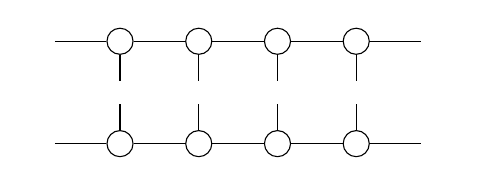
\begin{tikzpicture}
    \tikzmath{ \shift=0.3; };  % interval between up and down vertical lines

    %nodes at y=0
    \node[hidden] (head0) at (0,0) { };
    \node[circle]    (c1) at (1,0) { };
    \node[circle]    (c2) at (2,0) { };
    \node[circle]    (c3) at (3,0) { };
    \node[circle]    (c4) at (4,0) { };
    \node[hidden] (tail0) at (5,0) { };

    %nodes at y=1
    \node[hidden] (head1) at (0,1+\shift) { };
    \node[circle]    (c5) at (1,1+\shift) { };
    \node[circle]    (c6) at (2,1+\shift) { };
    \node[circle]    (c7) at (3,1+\shift) { };
    \node[circle]    (c8) at (4,1+\shift) { };
    \node[hidden] (tail1) at (5,1+\shift) { };


    %first line
    \draw[-] (head0.east)--(c1.west);
    \draw[-]    (c1.east)--(c2.west);
    \draw[-]    (c2.east)--(c3.west);
    \draw[-]    (c3.east)--(c4.west);
    \draw[-]    (c4.east)--(tail0.west);

    %second line
    \draw[-] (head1.east)--(c5.west);
    \draw[-]    (c5.east)--(c6.west);
    \draw[-]    (c6.east)--(c7.west);
    \draw[-]    (c7.east)--(c8.west);
    \draw[-]    (c8.east)--(tail1.west);

    % vertical lines
    \draw[-] (c1.north)--(1,0.5);
    \draw[-] (c2.north)--(2,0.5);
    \draw[-] (c3.north)--(3,0.5);
    \draw[-] (c4.north)--(4,0.5);

    \draw[-] (c5.south)--(1,0.5+\shift);
    \draw[-] (c6.south)--(2,0.5+\shift);
    \draw[-] (c7.south)--(3,0.5+\shift);
    \draw[-] (c8.south)--(4,0.5+\shift);

\end{tikzpicture}


\section*{}
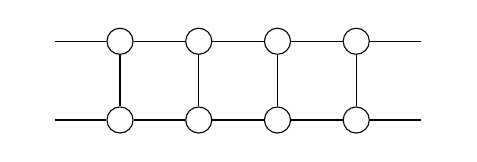
\begin{tikzpicture}
    %nodes at y=0
    \node[hidden] (head0) at (0,0) { };
    \node[circle]    (c1) at (1,0) { };
    \node[circle]    (c2) at (2,0) { };
    \node[circle]    (c3) at (3,0) { };
    \node[circle]    (c4) at (4,0) { };
    \node[hidden] (tail0) at (5,0) { };

    %nodes at y=1
    \node[hidden] (head1) at (0,1) { };
    \node[circle]    (c5) at (1,1) { };
    \node[circle]    (c6) at (2,1) { };
    \node[circle]    (c7) at (3,1) { };
    \node[circle]    (c8) at (4,1) { };
    \node[hidden] (tail1) at (5,1) { };

    %first line
    \draw[-] (head0.east)--(c1.west);
    \draw[-]    (c1.east)--(c2.west);
    \draw[-]    (c2.east)--(c3.west);
    \draw[-]    (c3.east)--(c4.west);
    \draw[-]    (c4.east)--(tail0.west);

    %second line
    \draw[-] (head1.east)--(c5.west);
    \draw[-]    (c5.east)--(c6.west);
    \draw[-]    (c6.east)--(c7.west);
    \draw[-]    (c7.east)--(c8.west);
    \draw[-]    (c8.east)--(tail1.west);

    % vertical lines
    \draw[-] (c1.north)--(c5.south);
    \draw[-] (c2.north)--(c6.south);
    \draw[-] (c3.north)--(c7.south);
    \draw[-] (c4.north)--(c8.south);
\end{tikzpicture}


\section*{}
\begin{align*}
    \left( 
        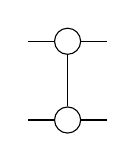
\begin{tikzpicture}[baseline=(current bounding box.center)]
            \node[circle] (c1) at (0,0) {};
            \node[circle] (c2) at (0,1) {};
            \draw[-] (c1.north)--(c2.south);
            \draw[-] (c1.west)--(-0.5,0);
            \draw[-] (c1.east)--(0.5,0);
            \draw[-] (c2.west)--(-0.5,1);
            \draw[-] (c2.east)--(0.5,1);
        \end{tikzpicture}
    \right)^M
\end{align*}


\section*{}
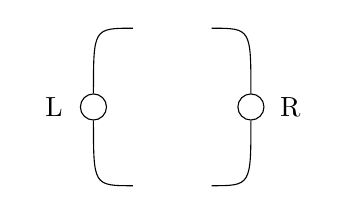
\begin{tikzpicture}
    %node and label
    \node[circle] (lp) at (0,0) {};
    \node[circle] (rp) at (2,0) {};
    \node[hidden] () at (-0.5,0) {L};
    \node[hidden] () at (2.5,0) {R};

    %curves
    \draw[] (lp.north) .. controls(0,1) .. (0.5,1);
    \draw[] (lp.south) .. controls(0,-1).. (0.5,-1);
    \draw[] (rp.north) .. controls(2,1) .. (1.5,1);
    \draw[] (rp.south) .. controls(2,-1).. (1.5,-1);

\end{tikzpicture}




\section{ $\Psi^\dagger \hat{H} \Psi$ }
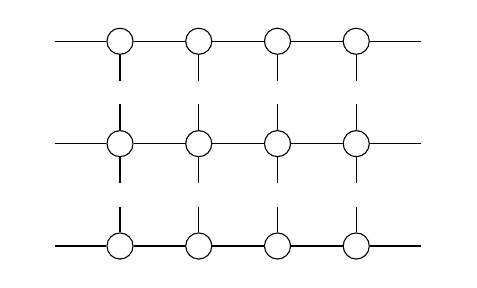
\begin{tikzpicture}
    \tikzmath{ \shift=0.3; };  % interval between up and down vertical lines

    %nodes at y=0
    \node[hidden] (head0) at (0,0) { };
    \node[circle]    (c1) at (1,0) { };
    \node[circle]    (c2) at (2,0) { };
    \node[circle]    (c3) at (3,0) { };
    \node[circle]    (c4) at (4,0) { };
    \node[hidden] (tail0) at (5,0) { };

    %nodes at y=1
    \node[hidden] (head1) at (0,1+\shift) { };
    \node[circle]    (c5) at (1,1+\shift) { };
    \node[circle]    (c6) at (2,1+\shift) { };
    \node[circle]    (c7) at (3,1+\shift) { };
    \node[circle]    (c8) at (4,1+\shift) { };
    \node[hidden] (tail1) at (5,1+\shift) { };

    %nodes at y=2
    \node[hidden] (head2) at (0,2+2*\shift) { };
    \node[circle]    (c9) at (1,2+2*\shift) { };
    \node[circle]   (c10) at (2,2+2*\shift) { };
    \node[circle]   (c11) at (3,2+2*\shift) { };
    \node[circle]   (c12) at (4,2+2*\shift) { };
    \node[hidden] (tail2) at (5,2+2*\shift) { };


    %line y=0
    \draw[-] (head0.east)--(c1.west);
    \draw[-]    (c1.east)--(c2.west);
    \draw[-]    (c2.east)--(c3.west);
    \draw[-]    (c3.east)--(c4.west);
    \draw[-]    (c4.east)--(tail0.west);

    %line y=1
    \draw[-] (head1.east)--(c5.west);
    \draw[-]    (c5.east)--(c6.west);
    \draw[-]    (c6.east)--(c7.west);
    \draw[-]    (c7.east)--(c8.west);
    \draw[-]    (c8.east)--(tail1.west);

    %line y=2
    \draw[-] (head2.east)--(c9.west);
    \draw[-]    (c9.east)--(c10.west);
    \draw[-]   (c10.east)--(c11.west);
    \draw[-]   (c11.east)--(c12.west);
    \draw[-]   (c12.east)--(tail2.west);

    % vertical lines
    \draw[-] (c1.north)--(1,0.5);
    \draw[-] (c2.north)--(2,0.5);
    \draw[-] (c3.north)--(3,0.5);
    \draw[-] (c4.north)--(4,0.5);

    \draw[-] (c5.south)--(1,0.5+\shift);
    \draw[-] (c6.south)--(2,0.5+\shift);
    \draw[-] (c7.south)--(3,0.5+\shift);
    \draw[-] (c8.south)--(4,0.5+\shift);

    \draw[-] (c5.north)--(1,1.5+\shift);
    \draw[-] (c6.north)--(2,1.5+\shift);
    \draw[-] (c7.north)--(3,1.5+\shift);
    \draw[-] (c8.north)--(4,1.5+\shift);

    \draw[-]  (c9.south)--(1,1.5+2*\shift);
    \draw[-] (c10.south)--(2,1.5+2*\shift);
    \draw[-] (c11.south)--(3,1.5+2*\shift);
    \draw[-] (c12.south)--(4,1.5+2*\shift);

\end{tikzpicture}


\section*{}
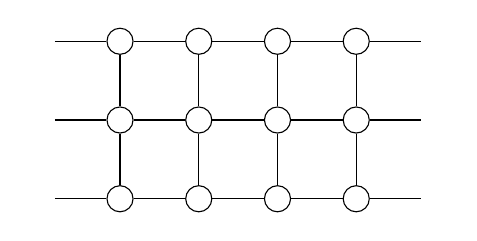
\begin{tikzpicture}
    \tikzmath{ \shift=0; };  % interval between up and down vertical lines

    %nodes at y=0
    \node[hidden] (head0) at (0,0) { };
    \node[circle]    (c1) at (1,0) { };
    \node[circle]    (c2) at (2,0) { };
    \node[circle]    (c3) at (3,0) { };
    \node[circle]    (c4) at (4,0) { };
    \node[hidden] (tail0) at (5,0) { };

    %nodes at y=1
    \node[hidden] (head1) at (0,1) { };
    \node[circle]    (c5) at (1,1) { };
    \node[circle]    (c6) at (2,1) { };
    \node[circle]    (c7) at (3,1) { };
    \node[circle]    (c8) at (4,1) { };
    \node[hidden] (tail1) at (5,1) { };

    %nodes at y=2
    \node[hidden] (head2) at (0,2) { };
    \node[circle]    (c9) at (1,2) { };
    \node[circle]   (c10) at (2,2) { };
    \node[circle]   (c11) at (3,2) { };
    \node[circle]   (c12) at (4,2) { };
    \node[hidden] (tail2) at (5,2) { };


    %line y=0
    \draw[-] (head0.east)--(c1.west);
    \draw[-]    (c1.east)--(c2.west);
    \draw[-]    (c2.east)--(c3.west);
    \draw[-]    (c3.east)--(c4.west);
    \draw[-]    (c4.east)--(tail0.west);

    %line y=1
    \draw[-] (head1.east)--(c5.west);
    \draw[-]    (c5.east)--(c6.west);
    \draw[-]    (c6.east)--(c7.west);
    \draw[-]    (c7.east)--(c8.west);
    \draw[-]    (c8.east)--(tail1.west);

    %line y=2
    \draw[-] (head2.east)--(c9.west);
    \draw[-]    (c9.east)--(c10.west);
    \draw[-]   (c10.east)--(c11.west);
    \draw[-]   (c11.east)--(c12.west);
    \draw[-]   (c12.east)--(tail2.west);

    % vertical lines
    \draw[-] (c1.north)--(c5.south);
    \draw[-] (c2.north)--(c6.south);
    \draw[-] (c3.north)--(c7.south);
    \draw[-] (c4.north)--(c8.south);

    \draw[-] (c5.north)-- (c9.south);
    \draw[-] (c6.north)--(c10.south);
    \draw[-] (c7.north)--(c11.south);
    \draw[-] (c8.north)--(c12.south);
\end{tikzpicture}



\section{$\Psi^\dagger \hat{H_2} \Psi$ }
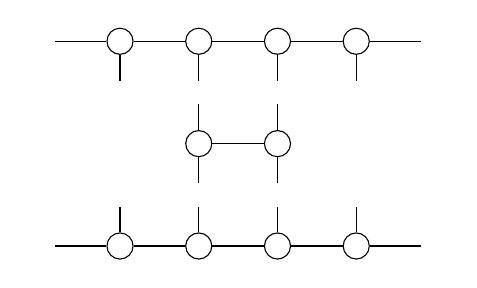
\begin{tikzpicture}
    \tikzmath{ \shift=0.3; };  % interval between up and down vertical lines

    %nodes at y=0
    \node[hidden] (head0) at (0,0) { };
    \node[circle]    (c1) at (1,0) { };
    \node[circle]    (c2) at (2,0) { };
    \node[circle]    (c3) at (3,0) { };
    \node[circle]    (c4) at (4,0) { };
    \node[hidden] (tail0) at (5,0) { };

    %nodes at y=1
    \node[hidden] (head1) at (0,1+\shift) { };
    \node[hidden]    (c5) at (1,1+\shift) { };
    \node[circle]    (c6) at (2,1+\shift) { };
    \node[circle]    (c7) at (3,1+\shift) { };
    \node[hidden]    (c8) at (4,1+\shift) { };
    \node[hidden] (tail1) at (5,1+\shift) { };

    %nodes at y=2
    \node[hidden] (head2) at (0,2+2*\shift) { };
    \node[circle]    (c9) at (1,2+2*\shift) { };
    \node[circle]   (c10) at (2,2+2*\shift) { };
    \node[circle]   (c11) at (3,2+2*\shift) { };
    \node[circle]   (c12) at (4,2+2*\shift) { };
    \node[hidden] (tail2) at (5,2+2*\shift) { };


    %line y=0
    \draw[-] (head0.east)--(c1.west);
    \draw[-]    (c1.east)--(c2.west);
    \draw[-]    (c2.east)--(c3.west);
    \draw[-]    (c3.east)--(c4.west);
    \draw[-]    (c4.east)--(tail0.west);

    %line y=1
    % \draw[-] (head1.east)--(c5.west);
    % \draw[-]    (1.5,1+\shift)--(c6.west);
    \draw[-]    (c6.east)--(c7.west);
    % \draw[-]    (c7.east)--(3.5,1+\shift);
    % \draw[-]    (c8.east)--(tail1.west);

    %line y=2
    \draw[-] (head2.east)--(c9.west);
    \draw[-]    (c9.east)--(c10.west);
    \draw[-]   (c10.east)--(c11.west);
    \draw[-]   (c11.east)--(c12.west);
    \draw[-]   (c12.east)--(tail2.west);

    % vertical lines
    \draw[-] (c1.north)--(1,0.5);
    \draw[-] (c2.north)--(2,0.5);
    \draw[-] (c3.north)--(3,0.5);
    \draw[-] (c4.north)--(4,0.5);

    % \draw[-] (c5.south)--(1,0.5+\shift);
    \draw[-] (c6.south)--(2,0.5+\shift);
    \draw[-] (c7.south)--(3,0.5+\shift);
    % \draw[-] (c8.south)--(4,0.5+\shift);

    % \draw[-] (c5.north)--(1,1.5+\shift);
    \draw[-] (c6.north)--(2,1.5+\shift);
    \draw[-] (c7.north)--(3,1.5+\shift);
    % \draw[-] (c8.north)--(4,1.5+\shift);

    \draw[-]  (c9.south)--(1,1.5+2*\shift);
    \draw[-] (c10.south)--(2,1.5+2*\shift);
    \draw[-] (c11.south)--(3,1.5+2*\shift);
    \draw[-] (c12.south)--(4,1.5+2*\shift);
\end{tikzpicture}


\section*{}
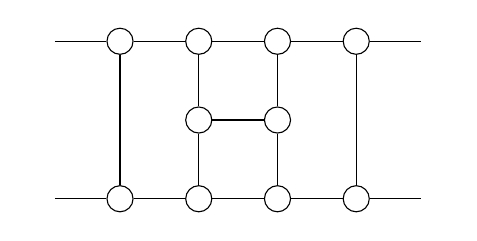
\begin{tikzpicture}
    \tikzmath{ \shift=0; };  % interval between up and down vertical lines

    %nodes at y=0
    \node[hidden] (head0) at (0,0) { };
    \node[circle]    (c1) at (1,0) { };
    \node[circle]    (c2) at (2,0) { };
    \node[circle]    (c3) at (3,0) { };
    \node[circle]    (c4) at (4,0) { };
    \node[hidden] (tail0) at (5,0) { };

    %nodes at y=1
    \node[hidden] (head1) at (0,1+\shift) { };
    \node[hidden]    (c5) at (1,1+\shift) { };
    \node[circle]    (c6) at (2,1+\shift) { };
    \node[circle]    (c7) at (3,1+\shift) { };
    \node[hidden]    (c8) at (4,1+\shift) { };
    \node[hidden] (tail1) at (5,1+\shift) { };

    %nodes at y=2
    \node[hidden] (head2) at (0,2+2*\shift) { };
    \node[circle]    (c9) at (1,2+2*\shift) { };
    \node[circle]   (c10) at (2,2+2*\shift) { };
    \node[circle]   (c11) at (3,2+2*\shift) { };
    \node[circle]   (c12) at (4,2+2*\shift) { };
    \node[hidden] (tail2) at (5,2+2*\shift) { };

    %line y=0
    \draw[-] (head0.east)--(c1.west);
    \draw[-]    (c1.east)--(c2.west);
    \draw[-]    (c2.east)--(c3.west);
    \draw[-]    (c3.east)--(c4.west);
    \draw[-]    (c4.east)--(tail0.west);

    %line y=1
    \draw[-]    (c6.east)--(c7.west);

    %line y=2
    \draw[-] (head2.east)--(c9.west);
    \draw[-]    (c9.east)--(c10.west);
    \draw[-]   (c10.east)--(c11.west);
    \draw[-]   (c11.east)--(c12.west);
    \draw[-]   (c12.east)--(tail2.west);

    % vertical lines
    \draw[-] (c1.north)--(c9.south);
    \draw[-] (c2.north)--(c6.south);
    \draw[-] (c3.north)--(c7.south);
    \draw[-] (c4.north)--(c12.south);

    \draw[-] (c6.north)--(c10.south);
    \draw[-] (c7.north)--(c11.south);

\end{tikzpicture}


\section*{}
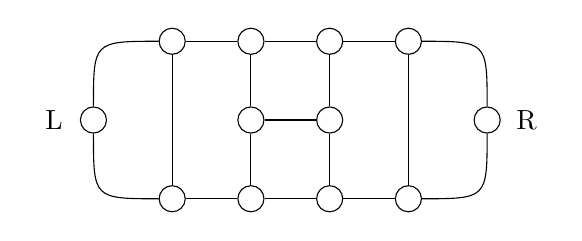
\begin{tikzpicture}
    \tikzmath{ \shift=0; };  % interval between up and down vertical lines

    %nodes at y=0
    \node[circle]    (c1) at (1,0) { };
    \node[circle]    (c2) at (2,0) { };
    \node[circle]    (c3) at (3,0) { };
    \node[circle]    (c4) at (4,0) { };

    %nodes at y=1
    \node[circle]    (c6) at (2,1) { };
    \node[circle]    (c7) at (3,1) { };

    %nodes at y=2
    \node[circle]    (c9) at (1,2) { };
    \node[circle]   (c10) at (2,2) { };
    \node[circle]   (c11) at (3,2) { };
    \node[circle]   (c12) at (4,2) { };


    %line y=0
    \draw[-]    (c1.east)--(c2.west);
    \draw[-]    (c2.east)--(c3.west);
    \draw[-]    (c3.east)--(c4.west);

    %line y=1
    \draw[-]    (c6.east)--(c7.west);

    %line y=2
    \draw[-]    (c9.east)--(c10.west);
    \draw[-]   (c10.east)--(c11.west);
    \draw[-]   (c11.east)--(c12.west);

    % vertical lines
    \draw[-] (c1.north)--(c9.south);
    \draw[-] (c2.north)--(c6.south);
    \draw[-] (c3.north)--(c7.south);
    \draw[-] (c4.north)--(c12.south);
    \draw[-] (c6.north)--(c10.south);
    \draw[-] (c7.north)--(c11.south);


    %left and right curves
    \node[circle] (lp) at (0,1) {};
    \node[circle] (rp) at (5,1) {};
    \node[hidden] () at (-0.5,1) {L};
    \node[hidden] () at  (5.5,1) {R};
    \draw[] (lp.north) .. controls(0,2) .. (c9.west);
    \draw[] (lp.south) .. controls(0,0) .. (c1.west);
    \draw[] (rp.north) .. controls(5,2) .. (c12.east);
    \draw[] (rp.south) .. controls(5,0) .. (c4.east);

\end{tikzpicture}

\end{document}